\documentclass{beamer}

\usetheme{Pk}

\newcommand\rb[1]{\textcolor{ThemeRed}{\textbf{#1}}}
\usepackage{listings}
\lstset{
  basicstyle=\scriptsize,
  columns=fullflexible,
  showstringspaces=false,
  commentstyle=\color{ThemeGrey}\upshape
}

\lstdefinelanguage{XML}
{
  morestring=[b]",
  moredelim=[s][\color{ThemeGreen}]{<}{\ },
  moredelim=[s][\color{ThemeGreen}]{</}{>},
  moredelim=[l][\color{ThemeGreen}]{/>},
  moredelim=[l][\color{ThemeGreen}]{>},
  stringstyle=\color{ThemeBlue},
  identifierstyle=\color{ThemeGreen},
  keywordstyle=\color{ThemeRed},
}


\title{Open Data Management \& Cloud\\exam project}
\subtitle{Audio music file archiving}
\author{Patrick Indri}
\date{\today}


\begin{document}
	\setcounter{showSlideNumbers}{0}

	\frame{\titlepage}

	\setcounter{framenumber}{0}
	\setcounter{showSlideNumbers}{1}


  \begin{frame}
    \frametitle{Introduction}

    \begin{block}{Aim of the project}
      Investigation of audio file archiving for music.
    \end{block}

    \vspace{1em}

    In particular:
    \begin{itemize}
      \item UML metadata model;
      \item XSD implementation and XML sample document;
      \item discussion of data discovery/access and interoperability;
      \item discussion of long term archiving and data preservation.
    \end{itemize}

    \vspace{1em}

    \rb{Data resource:} not an actual dataset but music files in general.

  \end{frame}



  \begin{frame}
    \frametitle{Metadata standards for audio files}
  \end{frame}



  \begin{frame}
    \frametitle{Model design}
  \end{frame}



  \begin{frame}
    \frametitle{UML}
    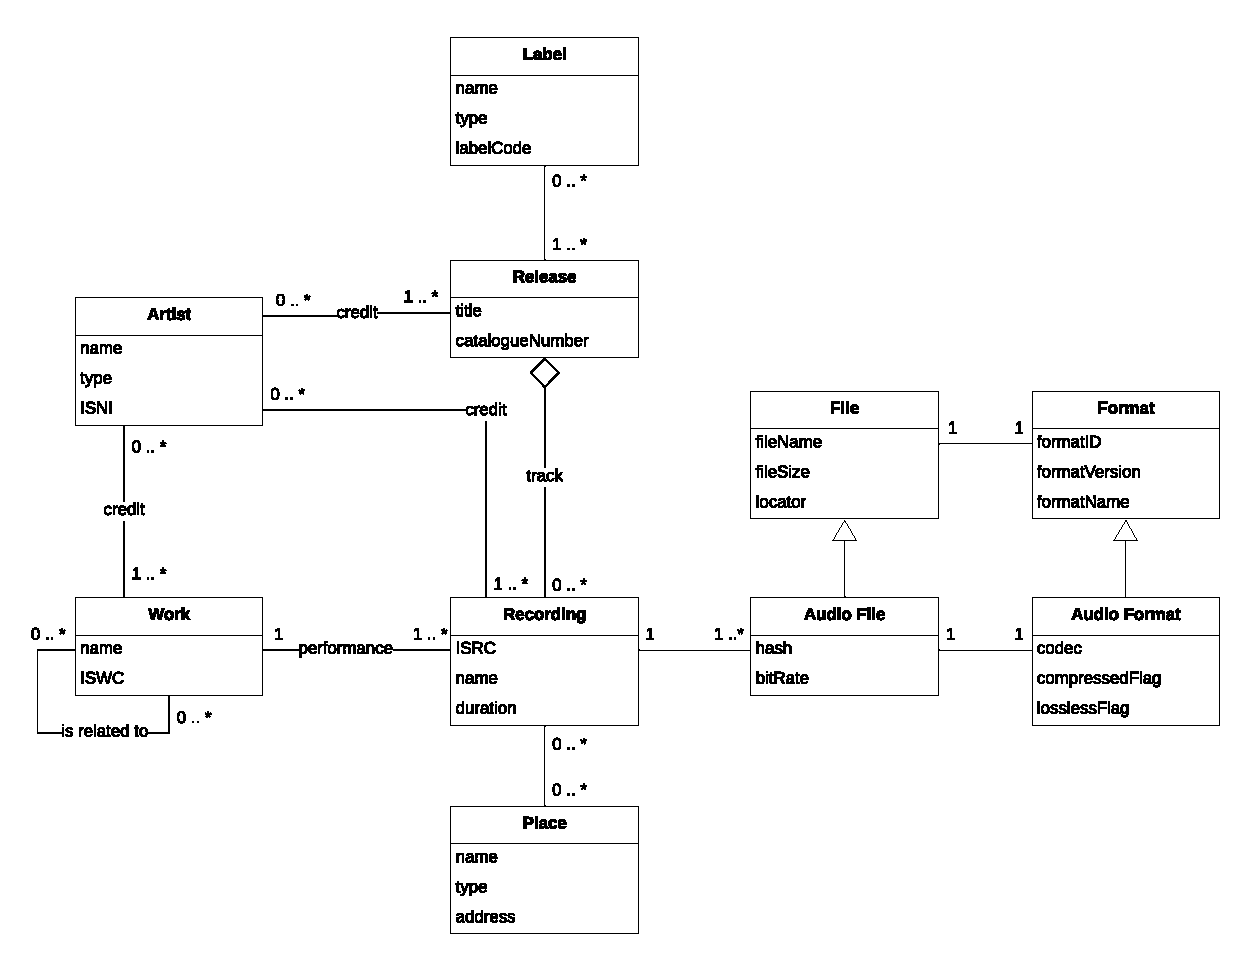
\includegraphics[width=1\textwidth]{img/UML.pdf}
  \end{frame}



  \begin{frame}
    \frametitle{XSD}
  \end{frame}



  \begin{frame}[fragile]
    \frametitle{XML example}
\lstset{basicstyle=\scriptsize}
\begin{lstlisting}[language=XML]
<work>
  <ISWC id="ISWC_T-000.000.000-A"></ISWC>
  <title lang="en">
    <dc:title>Test Work</dc:title>
  </title>
  <hasArtist label="Will Wilson" description="Singer">
  </hasArtist>
  <hasPerformance label="Test Rec." description="Studio Ver.">
    <relationIdentifier>
      <ISRC idref="ISRC_AAAAA0000000"></ISRC>
    </relationIdentifier>
  </hasPerformance>
</work>
\end{lstlisting}
  \end{frame}



\end{document}
